\chapter{ทฤษฎีและบทความที่เกี่ยวข้อง}
เนื่องจากการแบตเตอรี่นั้นมีองค์ประกอบและปัจจัยต่างๆที่ต้องทำการพิจารณาเพื่อนำไปพัฒนายานยนต์ไฟฟ้าต่อไปดังนั้นการเข้าใจส่วนประกอบ ปัจจัยต่างๆที่ส่งผลกระทบต่อแบตเตอรี่ คุณสมบัติของแบตเตอรี่ มีความสำคัญอย่างยิ่งเพื่อที่จะเข้าใจสิ่งเหล่านี้จึงมีการค้นคว้าวิจัยหาข้อมูลมากมาย ดังนั้นในหัวข้อนี้จึงได้ทำการรวบรวมข้อมูล ทฤษฎีที่เกี่ยวข้องงานวิจัยต่างๆที่ใช้อ้างอิงสำหรับโครงงานนี้แล้วคือ
%===========================================================================================
\section{แบตเตอรี่ลิเธียมไอออน}
คำนิยามของแบตเตอรี่ลิเธียมไอออนนั้นไม่ได้มีการบัญญัติขึ้นอย่างเป็นทางการแต่โดยทั่วไปแล้วแบตเตอรี่ลิเธียมไอออนสามารถนิยามได้ว่าเป็นระบบกักเก็บพลังงานซึ่งอาศัยปฏิกริยาจากขั้วทางไฟฟ้าทั้งสองโดยที่มีลิเธียมไอออน(Li+)ทำหน้าที่เป็นตัวนำประจุ ซึ่งจากนิยามของแบตเตอรี่ลิเธียมไอออนข้างต้นนี้ไม่ได้หมายถึงแบตเตอรี่เพียงชนิดเดียวยกตัวอย่างเช่น แบตเตอรี่ตะกั่ว-กรดหรือแบตเตอรี่นิเกิลแคดเมียมที่หมายถึงแบตเตอรี่ชนิดนั้นๆโดยสรุปจากคุณสมบัติทางเคมีของเซลล์แบตเตอรี่
แบตเตอรี่ลิเธียมไอออนนั้นมีหลายคุณสมบัติทางเคมีโดยความแตกต่างนี้ขึ้นอยู่กับวัสดุส่วนประกอบของเซลล์แบตเตอรี่ซึ่งความแตกต่างของส่วนประกอบทำให้ได้แบตเตอรี่ลิเธียมไอออนหลายชนิดและแบตเตอรี่ลิเธียมไอออนนั้นยังมี
หลายรูปแบบหรือรูปร่างในขณะที่หลักการทำงานนั้นยังคงตามนิยามที่ได้กล่าวไว้ข้างต้นซึ่งหลักการทำงานความแตกต่างทางรูปร่างและชนิดนี้จะอธิบายในหัวข้อถัดไป
%============================================================================================
\subsection{โครงสร้างและส่วนประกอบ}
หัวข้อนี้จะอธิบายถึงโครงสร้าง ส่วนประกอบหลัก และวัสดุที่นำมาเป็นส่วนประกอบหลักอย่างคร่าวๆของเซลล์แบตเตอรี่ลิเธียมไอออนจากรูปที่\ref{fig:Li-ion Structure} เซลล์แบตเตอรี่ลิเธียมไอออนแบบทรงกระบอกนั้นจะประกอบไปด้วย ขั้วบวก(แคโทด)ขั้วลบ(แอโนด)ตัวรับกระแสขั้วลบ ตัวรับกระแสขั้วบวก อิเล็กโทรไลต์และฉนวนระหว่างขั้วทั้งสองโดยทั่วไปแล้วขั้วบวกนั้นทำจากสารประกอบลิเธียมไอออนเช่น LiCoO2, LiNiO2, LiMn2O4, LiFePO4 และ LiNixCo1-2xMnxO2 ส่วนขั้วลบโดยทั่วไปทำจาก Li4Ti5O12, LixC6, TiS2 และ V2O5 อิเล็กโทรไลต์ใช้เกลือลิเธียมเช่น LiPF6, LiBF4, LiClO4, และ LiAsF6 ซึ่งละลายในสารละลายอินทรีย์เช่น ethylene carbonate (EC), propylene carbonate (PC), dimethyl carbonate (DMC) และ chlorine methyl carbonate (ClMC) สุดท้ายฉนวนระหว่างขั้วทั้งสองเช่น polyethylene (PE) และ polypropylene (PP) จะเห็นได้ว่ามีวัสดุหลายอย่างมากที่สามารถนำมาใช้เป็น ขั้วบวกของแบตเตอรี่ ขั้วลบของแบตเตอรี่ อิเล็กโทรไลต์ และฉนวนที่กั้นระหว่างขั้วทั้งสองซึ่งข้อจำกัดทางเทคโนโลยีของวัสดุต่างๆนั้นคือจะต้องสามารถทำงานตามแนวทางดังนี้
\begin{center}
	\begin{figure}[!h]
		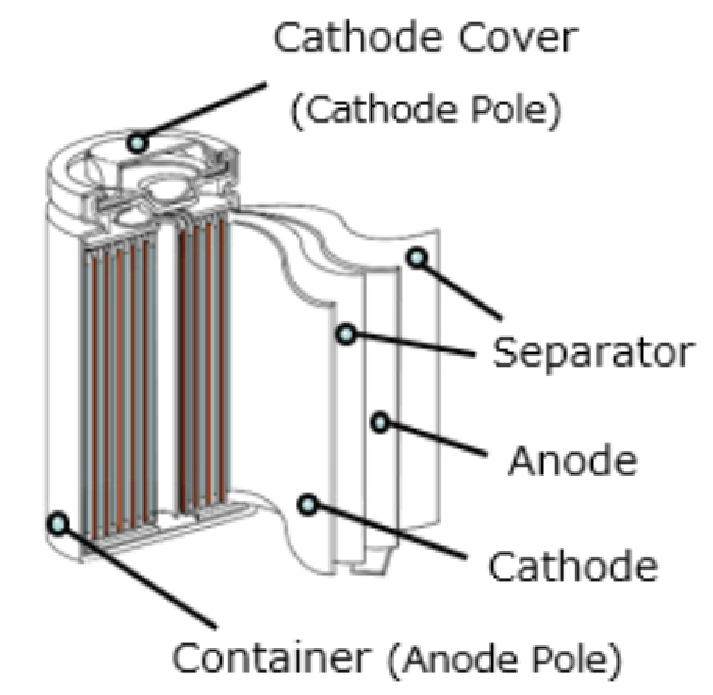
\includegraphics[width=0.4\linewidth]{Chapters/img/Cyrinder_battery.pdf}
		\centering
		\captionsetup{justification=centering,margin=2cm}
		\caption{โครงสร้างของเซลล์แบตเตอรี่ลิเธียมไอออนแบบทรงกระบอก}
		\label{fig:Li-ion Structure}
	\end{figure}
\end{center}
\begin{itemize}
 {\item 
 	อิเล็กโทรไลต์นั้นจะต้องสามารถส่งผ่านลิเธียมไอออนได้มากที่สุดเท่าที่สามารถส่งผ่านได้ภายใต้เงื่อนไขคือแบตเตอรี่นั้นจะต้องสามารถทำงานในสภาพแวดล้อมทั่วไปได้เช่นสามารถทำงานได้ในช่วงอุณหภูมิ -30$^\circ C$ 	 	     เพื่อที่ยานยนต์นั้นสามารถจอดได้ในกรณีที่จอดในช่วงเวลาที่อุณหภูมินั้นเย็นจัดจนถึงอุณหภูมิ +60$^\circ C$ ในกรณีที่อุณหภูมิของแบตเตอรี่นั้นสูงขึ้นเนื่องจากเป็นผลมาจากสภาพแวดล้อมภายนอกและเป็นผลมาจากการชาร์จ}
 {\item 
 	ในทำนองเดียวกันฉนวนที่กั้นระหว่างขั้วทั้งสองนั้นจะต้องสามารถส่งผ่านลิเธียมไอออนได้มากที่สุดเท่าที่จะสามารถทำได้ภายใต้เงื่อนไขเดียวกันกับอิเล็กโทรไลต์และจะต้องมีความสามารถทนความร้อนสูงแบบฉับพลัน
 }
 {\item 
 	ความเข้ากันได้ของวัสดุของขั้วของแบตเตอรี่นั้นจะต้องสามารถทำให้แบตเตอรี่มีความจุมากที่สุดเท่าที่จะสามารถเป็นไปได้โดยข้อสรุปของวัสดุต่างๆและปฏิกิริยาทางเคมีไฟฟ้านั้นเป็นไปดังรูปที่ 2 	       และแรงดันของเซลล์แบตเตอรี่นั้นขึ้นอยู่ความแตกต่างระหว่างคู่วัสดุที่ใช้นำมาทำเป็นขั้วของแบตเตอรี่ซึ่งแรงดันนั้นอาจจะถูกเปลี่ยนแปลงไปเนื่องจากการสูญเสียภายในเซลล์แบตเตอรี่อย่างเช่น การสูญเสีย IR losses เนื่องจากความสามารถในการส่งผ่านลิเธียมไอออนที่ไม่ดีในอิเล็กโทรไลท์ยกตัวอย่างเช่นถ้า LiFePO4 นั้นถูกใช้นำมาเป็นขั้วบวกและ Li4Ti5O12 เป็นขั้วลบของแบตเตอรี่จะทำให้ได้แรงดันเปิดวงจรปกตินั้นคือ$V_{oc}=V^+-V^-=1.95\ V$ โดย $V^+$ นั้นแทนศักย์ไฟฟ้าทางขั้วบวกของแบตเตอรี่ส่วน $V^-$ แทนศักย์ไฟฟ้าทางขั้วลบของแบตเตอรี่
 }
\end{itemize}

%===================================================================================================

\subsection{หลักการทำงานของแบตเตอรี่ลิเธียมไอออน}
\begin{center}
	\begin{figure}[!h]
		\includegraphics[width=0.6\linewidth]{Chapters/img/battery_structure.png}
			\centering
			\captionsetup{justification=centering,margin=2cm}
			\caption{ส่วนประกอบและการทำงานของเซลล์แบตเตอรี่ลิเธียมไอออน}
			\label{fig:Battery_Struc}
	\end{figure}
\end{center}

จากรูปที่\ref{fig:Battery_Struc} เป็นการทำงานของเซลล์แบตเตอรี่ลิเธียมไอออนในสภาวะการทำงานทั้งสองสภาวะดังนี้
\begin{itemize}
	{\item
		เมื่อเซลล์แบตเตอรี่อยู่ในสภาวะดิสชาร์จหรือทำงานเป็นแหล่งจ่ายพลังงาน อิเล็กตรอนจะเคลื่อนย้ายจากขั้วแอโนดผ่านตัวรับกระแสทั้งสองด้านและโหลดไปยังขั้วแคโทดในขณะเดียวกัน Li+ เคลื่อนย้ายจากขั้วแอโนดผ่านอิเล็กโทรไลต์และฉนวนไปยังขั้วแคโทด}
	{\item
		ในทางกลับกันเมื่อเซลล์แบตเตอรี่อยู่ในสภาวะการชาร์จ อิเล็กตรอนจะเคลื่อนย้ายจากขั้วแคโทดผ่านแหล่งจ่ายและตัวรับกระแสไปยังขั้วแอโนดในขณะเดียวกัน Li+ เคลื่อนย้ายจากขั้วแคโทดผ่านอิเล็กโทรไลต์และฉนวนไปยังขั้วแอโนด}
\end{itemize}
 ซึ่งเพื่อคงความเป็นกลางทางไฟฟ้าการเคลื่อนย้ายของอิเล็กตรอนและ Li+ นั้นจึงเกิดขึ้นพร้อมกันและเนื่องจากการเคลื่อนย้ายของอิเล็กตรอนก็มีผลทำให้เกิดกระแสไฟฟ้า
\newline ยกตัวอย่างเช่น พิจารณาแบตเตอรี่ลิเธียมแมงกานีสออกไซด์ (Lithium Manganese Oxide, LMO) เมื่อแบตเตอรี่อยู่ในสภาวะการชาร์จ Li+ เคลื่อนย้ายออกจาก LiMn2O4 ที่เป็นสารประกอบของขั้วแคโทดผ่านอิเล็กโทรไลต์และฉนวนไปสะสมอยู่ที่ชั้นคาร์บอนของกราไฟท์ที่เป็นขั้วแอโนดในทางตรงกันข้ามเมื่ออยู่ในสภาวะการดิสชาร์จ Li+ ที่สะสมอยู่ที่ชั้นคาร์บอนของกราไฟท์จากการชาร์จเคลื่อนย้ายผ่านอิเล็กโทรไลต์และฉนวนไปยัง LiMn2O4 ซึ่งปฏิกริยาที่เกิดขึ้นนี้เป็นดังนี้
 \newline ปฏิกิริยาทางขั้วแอโนด
\begin{equation}
LiMn_{2}O_{4} \Leftrightarrow Li_{1-x}Mn_{2}O_{4}+xLi^{+}+xe^{-} \label{eq:1}
\end{equation}
 \newline ปฏิกิริยาทางขั้วแคโทด
\begin{equation}
C+xLi^{+}+xe^{-} \Leftrightarrow Li_{x}C \label{eq:2}
\end{equation}
\newline ปฏิกิริยาทั้งระบบ
\begin{equation}
LiMn_{2}O_{4}+C \Leftrightarrow Li_{1-x}Mn_{2}O_{4}+Li_{x}C \label{eq:3}
\end{equation}
%===================================================================================================
\subsection{ลักษณะของแบตเตอรี่ลิเธียมไอออน}
เซลล์แบตเตอรี่ลิเธียมไอออนมีรูปลักษณ์ภายนอกที่นิยมในท้องตลาดอยู่ 3 ลักษณะดังนี้ ทรงกระบอก ทรงกล่อง และแบบแผ่น ซึ่งภายในจะมีลักษณะเป็นแบบพันรอบหรือแบบชั้นนั้นจะขึ้นอยู่กับลักษณะภายนอก
ตัวถังภายนอกของเซลล์แบตเตอรี่นั้นทำจากโลหะเช่น สแตนเลสหรืออลูมิเนียมสำหรับเซลล์แบบทรงกระบอกและทรงกล่อง อลูมิเนียมแผ่นสำหรับเซลล์แบบแผ่น ตัวถังของเซลล์แบตเตอรี่มีหน้าที่ที่สำคัญมากกว่าเป็นเพียงแค่ภาชนะบรรจุส่วนประกอบภายในซึ่งหน้าที่ที่สำคัญมากอย่างแรกนั่นคือป้องกันส่วนประกอบภายในจากความชื้นและแก็สออกซิเจนจากภายนอกซึ่งกัดกร่อนหรือทำให้ขั้วของเซลล์นั้นเป็นสนิม
และทำหน้าที่เป็นฉนวนระหว่างขั้วบวกและขั้วลบระหว่างเซลล์แบตเตอรี่หน้าที่ที่สำคัญอีกอย่างหนึ่งของตัวถังนั่นคือลดความดันจากภายในของเซลล์แบตเตอรี่ในขณะที่เซลล์ทำงานผิดปกติจนอาจทำให้ผิดรูปร่างทั้งนี้เพื่อให้ยังคงพื้นที่สำหรับเซลล์แบตเตอรี่
ในโมดูลแบตเตอรี่แต่สำหรับตัวถังแบบแผ่นนั้นไม่สามารถทำได้
\newline\hspace*{2cm} ดังตารางที่\ref{tab:compare_shape} เป็นการสรุปโดยสังเขปของเซลล์แบตเตอรี่ทั้ง 3 ลักษณะทั้งนี้เซลล์แบตเตอรี่แต่ละแบบนั้นมีข้อดีและข้อเสียแตกต่างกันแล้วแต่การนำไปประยุกต์ใช้
%Table 1
%\begin{center}
%	\begin{figure}[!h]
%		\includegraphics[width=0.6\linewidth]{Chapters/img/Compare_Cell.png}
%			\centering
%			\captionsetup{justification=centering,margin=2cm}
%			\caption{เป็นการสรุปโดยสังเขปของเซลล์แบตเตอรี่ทั้ง 3 ลักษณะทั้งนี้เซลล์แบตเตอรี่แต่ละแบบนั้นมีข้อดีและข้อเสียแตกต่างกันแล้วแต่การนำไปประยุกต์ใช้}
%	\end{figure}
%\end{center}
\begin{table}[H]
\caption{ตารางเปรียบเทียบรูปร่างเซลล์แบตเตอรี่อย่างง่าย}
\centering
\begin{tblr}{
  cells={valign=m,halign=c},
  row{1}={font=\bfseries,rowsep=8pt},
  column{1} = {5cm}
}
%\begin{tabular}{ | c c c c | }
%	\hline \\
      รูปร่าง & แบบทรงกระบอก & แบบทรงสี่เหลี่ยม & แบบซอง \\ \hline
 	&
 	\includegraphics[scale=0.5,valign=c]{Chapters/img/Cyrinder_battery_table.png}
 	&
 	\includegraphics[scale=0.5,valign=c]{Chapters/img/Prismatic_battery.png}
 	&
	\includegraphics[scale=0.5,valign=c]{Chapters/img/Pounch_battery.png} \\
	การจัดวางขั้วของแบตเตอรี่ & พันรอบ & พันรอบ & วางซ้อน\\
	ความแข็งแรงทางกล & ++ & + & -\\
	การระบายความร้อน & - & + & +\\
	พลังงานจำเพาะ & + & + & ++\\
	ความหนาแน่นพลังงาน & + & ++ & + \\ \hline
%\end{tabular}
\end{tblr}
\label{tab:compare_shape}
\end{table}
%================================================================================================
\subsection{คุณลักษณะของแบตเตอรี่ลิเธียมไอออน}
ในหัวข้อนี้จะสรุปคำศัพท์หรือคุณลักษณะต่างๆที่ใช้ในการระบุ เปรียบเทียบ และจำแนกแบตเตอรี่ลิเธียมไอออนซึ่งเป็นพื้นฐานสำคัญดังนี้
\begin{itemize}
	{\item
		C rate และ E rate กระแสดิสชาร์จบ่อยครั้งจะแสดงอยู่ใน C-rate ซึ่ง C-rate คืออัตราการดิส-ชาร์จต่อความจุสูงสุดของแบตเตอรี่เช่น 1C      	  หมายถึงกระแสดิสชาร์จนี้จะดิสชาร์จแบตเตอรี่หมดภายใน 1 ชั่วโมงสำหรับแบตเตอรี่ 100Ah กระแสดิสชาร์จจะเท่ากับ 100A ที่ 5C นั้นกระแสดิสชาร์จจะอยู่ที่ 500A และที่ C/2 
		กระแสดิสชาร์จจะอยู่ที่ 50A ในทำนองเดียวกัน E-rate คืออัตราพลังงานไฟฟ้าดิสชาร์จ 1E หมายถึงพลังงานไฟฟ้าที่ใช้ในการดิสชาร์จหมดภายใน 1 ชั่วโมง}
	{\item
		State of Charge (SOC) หมายถึงการแสดงสถานะความจุของแบตเตอรี่เทียบกับความจุสูงสุดของแบตเตอรี่เป็นเปอร์เซ็นต์}
	{\item
		Depth of Discharge (DOD) หมายถึงเปอร์เซ็นต์ความจุของแบตเตอรี่ที่ถูกดิสชาร์จไปเทียบกับความจุสูงสุดของแบตเตอรี่}
	{\item
		แรงดันที่ขั้ว (Terminal Voltage) หมายถึงแรงดันระหว่างขั้วของแบตเตอรี่ในขณะต่อโหลดซึ่งแรงดันนั้นขึ้นอยู่กับ SOC และกระแสชาร์จหรือดิสชาร์จ}
	{\item
		แรงดันเปิดวงจร (Open-circuit Voltage, OCV) หมายถึงแรงดันระหว่างขั้วของแบตเตอรี่ในขณะที่ไม่มีโหลดซึ่งขึ้นอยู่กับ SOC เช่นกัน}
	{\item
		แรงดันปกติ (Nominal Voltage) หมายถึงการรายงานแรงดันของแบตเตอรี่หรือแรงดันอ้างอิงของแบตเตอรี่}
	{\item
		แรงดันตัด (Cut-off Voltage) หมายถึงแรงดันต่ำที่สุดที่แบตเตอรี่สามารถจ่ายได้หรือหมายถึงแรงดันที่แสดงถึงสถานะของแบตเตอรี่ที่หมดแล้ว}
	{\item
		ความจุหรือความจุปกติ (Capacity or Nominal Capacity, Ah) หมายถึงความจุคูลอมบิกเมตริกหรือก็คือแอมแปร์ชั่วโมงทั้งหมดที่แบตเตอรี่สามารถดิสชาร์จได้จาก 100\%SOC จนถึงแรงดันตัด}
	{\item
		พลังงานหรือพลังงานปกติ (Energy or Nominal Energy, Wh) หมายถึงความจุพลังงานของแบตเตอรี่หรือก็คือวัตต์ทั้งหมดที่แบตเตอรี่สามารถดิสชาร์จได้จาก 100\%SOC จนถึงแรงดันตัด}
	{\item
		ไลฟ์ไซเคิล (Cycle Life) หมายถึงจำนวนรอบในการดิสชาร์จของแบตเตอรี่ที่สามารถดิสชาร์จได้ก่อนที่จะเสื่อมสภาพตามเกณฑ์อย่างไรก็ตามสภาพการทำงานของแบตเตอรี่นั้นมีปัจจัยหลายอย่างนอกจากจำนวนรอบการดิสชาร์จเช่น ความชื้นและอุณหภูมิ}
	{\item
		พลังงานจำเพาะ (Specific Energy, Wh/kg) หมายถึงพลังงานปกติต่อมวลของแบตเตอรี่บางครั้งอาจจะหมายถึงความหนาแน่นพลังงานโดยน้ำหนักของแบตเตอรี่}
	{\item
		กำลังไฟฟ้าจำเพาะ (Specific Power, W/kg) หมายถึงกำลังไฟฟ้าสูงสุดต่อมวลของแบตเตอรี่}
	{\item
		ความหนาแน่นพลังงาน (Energy Density, Wh/L) หมายถึงพลังงานปกติต่อหนึ่งหน่วยปริมาตรบางครั้งอาจจะหมายถึงความหนาแน่นพลังงานโดยปริมาตร}
	{\item
		ความหนาแน่นกำลังไฟฟ้า (Power Density, W/L) หมายถึงกำลังไฟฟ้าสูงสุดต่อหนึ่งหน่วยปริมาตรของแบตเตอรี่}
	{\item
		กระแสดิสชาร์จต่อเนื่องสูงสุด (Maximum Continuous Discharge Current) หมายถึงกระ-แสดิสชาร์จสูงสุดที่แบตเตอรี่สามารถดิสชาร์จได้อย่างต่อเนื่องข้อจำกัดนี้จะถูกกำหนดโดยโรงงานแบตเตอรี่เพื่อป้องกันอัตราการดิสชาร์จที่มากเกินไปซึ่งอาจจะทำให้แบตเตอรี่เสียหายหรือลดความจุลงได้}
	{\item
		กระแสพัลส์สูงสุดใน 30 วินาที (Maximum 30-sec Discharge Pulse Current) หมายถึงกระแสดิสชาร์จสูงสุดฉับพลันโดยดิสชาร์จเป็นเวลา 30 วินาที}
	{\item
		แรงดันชาร์จ (Charge Voltage) หมายถึงแรงดันของแบตเตอรี่เมื่อแบตเตอรี่ชาร์จเต็มแล้ว}
	{\item
		แรงดันลอยตัว (Float Voltage) หมายถึงแรงดันคงที่ที่แบตเตอรี่ชาร์จจนเต็มแล้วก่อนที่จะเกิดการดิสชาร์จเองภายใน}
\end{itemize}
%====================================================================================================
\subsection{แบตเตอรี่ลิเธียมไอออนชนิดต่างๆ}
	ในหัวข้อนี้จะกล่าวถึง สรุปข้อแตกต่าง ของแบตเตอรี่ลิเธียมไอออนแต่ละชนิดแบตเตอรี่ลิเธียมไอออนในปัจจุบันนั้นเป็นที่นิยมกันอยู่ในตลาดทั้งสิ้น 6 ชนิดซึ่งแต่ละชนิดนั้นโดยทั่วไปแล้วจะจำแนกตวามวัสดุที่นำมาใช้เป็นขั้วบวกของแบตเตอรี่ยกเว้นแบตเตอรี่ลิเธียมไอออนชนิดิเธียมไท-ทาเนต(Lithium Titanate, LTO) ที่ใช้วัสดุที่ใช้นำมาเป็นขั้วลบคือ Li4Ti5O12 มาทำการจำแนก ซึ่งแบตเตอรี่ลิเธียมไอออนทั้ง 6 ชนิดที่ได้อ้างถึงมีด้วยกันดังนี้ 
\subsubsection*{แบตเตอรี่ลิเธียมโคบอลต์ออกไซด์\\ (Lithium Cobalt Oxide Battery)}
	แบตเตอรี่ลิเธียมโคบอลต์ออกไซด์ถูกพัฒนาขึ้นครั้งแรกโดยบริษัท Sony ในปี 1991 แบตเตอรี่ลิเธียมโคบอลต์ออกไซด์ถูกใช้กับอุปกรณ์อิเล็กทรอนิกส์ส่วนตัวเป็นส่วนใหญ่เช่น แล็ปท็อป กล้องถ่ายรูป ฯลฯ เป็นต้นเนื่องจากมีความหนาแน่นของพลังงานสูง อายุการใช้งานนาน และผลิตง่าย แต่แบตเตอรี่ลิเธียมโคบอลต์ออกไซด์นั้นมีปฏิกิริยาสูงดังนั้นจึงทำให้ไม่เสถียรทางความร้อนและต้องการการวัด ตรวจจับ แสดงผลตลอดช่วงเวลาทำงานเพื่อความปลอดภัยและเนื่องจากโคบอลต์นั้นเป็นวัสดุที่หาได้ยากทำให้แบตเตอรี่ลิเธียมโคบอลต์ออกไซด์มีราคาแพงและด้วยปัญหาด้านความร้อนแบตเตอรี่ลิเธียมโคบอลต์ออกไซด์จึงไม่ค่อยเหมาะกับการนำไป
ใช้ในยานยนต์ไฟฟ้า
\newline\hspace*{2cm}
อย่างไรก็ตามแบตเตอรี่ลิเธียมโคบอลต์ออกไซด์นั้นได้ถูกนำไปใช้กับยานยนต์ไฟฟ้าอย่าง Tesla Roadster และ Smart Fortwo Electric drive(ED)
\subsubsection*{แบตเตอรี่ลิเธียมแมงกานีสออกไซด์\\ (Lithium Manganese Oxide Battery, LMO)}
	แบตเตอรี่ลิเธียมแมงกานีสออกไซด์ได้ถูกนำเสนอขึ้นเป็นครั้งแรกในช่วงต้นทศวรรษ 1980 และใช้เวลากว่า 15 ปีกว่าจะนำมาจำหน่ายในท้องตลาด ด้วยสถาปัตยกรรมโครงสร้างทางด้านเคมีช่วยเพิ่มการเคลื่อนย้ายของไอออน(Li+)ในอิเล็กโทรดเป็นผลทำให้ลดความต้านทานภายในของแบตเตอรี่และช่วยให้ทนกระแสไฟฟ้าได้มากขึ้นนั่นหมายความว่าสามารถเพิ่มความเร็วในการชาร์จหรือเพิ่มกระแสไฟฟ้าในการชาร์จและสามารถใช้กระแสดิสชาร์จที่สูงได้ ซึ่งข้อดีทางเคมีนี้ทำให้แบตเตอรี่ลิเธี-ยมแมงกานีสออกไซด์นั้นมีเสถียรภาพทาทงด้านความร้อนมากกว่าแบตเตอรี่ลิเธียมโคบอลต์ออกไซด์แต่มีข้อเสียนั่นคือมีความจุน้อยและอายุการใช้งานสั้นกว่าโดยประมาณ 33\% 
\newline\hspace*{2cm}ส่วนมากแบตเตอรี่ลิเธียมแมงกานีสออกไซด์นั้นถูกผสมเข้ากับแบตเตอรี่ลิเธียมแมงกานีสโคบอลต์ออกไซด์เพื่อเพิ่มพลังงานจำเพาะและอายุการใช้งานซึ่งแบตเตอรี่โดยการผสมนี้ในอดีตเคยถูกใช้ในยานยนต์ไฟฟ้าหลายรุ่นเช่น Nissan Leaf, Chevy volt, BMW i3
\subsubsection*{แบตเตอรี่ลิเธียมฟอสเฟต\\ (Lithium Iron Phosphate, LFP)}
	ในปี 1996 กลุ่มนักวิจัยในมหาวิทยาลัยเทกซัสออสติน(The University of Texas at Austin) ค้นพบว่าฟอสเฟตนั้นสามารถนำมาใช้เป็นอิเล็กโทรดของแบตเตอรี่ลิเธียมไอออนได้ ฟอสเฟตนั้นช่วยให้มีความสเถียรต่อการชาร์จเกิน(Over charge)และช่วยเพิ่มความทนทานต่อความร้อน แบตเตอรี่ลิเธียมฟอสเฟตมีความสามารถทางเคมีไฟฟ้าที่ดีเช่น มีความต้านทานต่ำ เป็นต้น มีช่วงอุณหภูมิการทำงานที่กว้างคือ +60$^{\circ}C$ ถึง -30$^{\circ}C$ และเกิดปฏิกิริยาคายความร้อนสูง(Thermal runaway)ได้ยากแต่มีการดิสชาร์จเองสูงมากกว่าแบตเตอรี่ลิเธียมไอออนชนิดอื่นๆทำให้มีปัญหาทางด้านสมดุลของอายุแบตเตอรี่ซึ่งสามารถใช้อุปกรณ์อิเล็กทรอนิกส์มาช่วยควบคุมปัญหานี้ได้เช่น BMS แต่ก็ทำให้ราคาของแบตเตอรี่นั้นสูงขึ้น
\newline\hspace*{2cm}
ด้วยประสิทธิภาพอัตราส่วนกำลังไฟฟ้าต่อน้ำหนักและความปลอดภัยสูงนั่นทำให้แบตเตอรี่ลิเธียมฟอสเฟตนิยมใช้มากในรถบ้าน มีการร่วมมือกันระหว่างบริษัทในประเทศเยอรมันได้แก่ ElektroFahrzeuge Stuttgart และ WOF ได้ทำรถบ้านที่ใช้ระบบไฟฟ้าทั้งหมดเจ้าแรกส่งออกสู่ตลาดซึ่งในระบบไฟฟ้านี้ก็นำแบตเตอรี่ลิเธียมมาใช้ด้วยเช่นกัน
\subsubsection*{เเบตเตอรี่ลิเธียมนิกเกิลแมงกานีสโคบอลต์ออกไซด์\\ (Lithium Nickel Manganese Cobalt Oxide Battery, NMC)}
	แบตเตอรี่นิกเกิลแมงกานีสโคบอลต์ออกไซด์สามรถออกแบบให้มีพลังงานจำเพาะสูงหรือกำลังไฟฟ้าได้ซึ่งเป็นผลดีมาจากการผสมกันระหว่างโลหะ 2 ชนิดคือนิกเกิลและแมงกานีส นิกเกิลนั้นทำให้พลังงานจำเพาะสูงแต่มีความเสถียรต่ำส่วนแมงกานีสนั้นทำให้ความต้านทานภายในต่ำแต่มี
	\\ข้อเสียคือทำให้พลังงานจำเพาะต่ำซึ่งอัตราส่วนของผสมโลหะต่างๆของแบตเตอรี่ลิเธียมนิกเกิลแมงกานีสโคบอลต์ออกไซด์นั้นขึ้นอยู่กับแต่ละโรงงานผลิตซึ่งมีดังนี้ NMC111(ความจุ 154 $Ah\cdot kg^{-1}$ ที่ 0.1C) NMC442 NMC622 และในปัจจุบัน NMC811(ความจุ > 185 $Ah\cdot kg^{-1}$ ที่ 0.1C)	
\newline\hspace*{2cm}การผสมกันระหว่างแมงกานีสและนิกเกิลช่วยเสริมข้อดีของกันและกันทำให้แบตเตอรี่ลิเธียมนิเกิลแมงกานีสโคบอลต์ออกไซด์เป็นแบตเตอรี่ลิเธียมไอออนที่ประสบความสำเร็จมากที่สุดและเหมาะสำหรับการนำไป
	ใช้กับยานยนต์ไฟฟ้าซึ่งปัจจุบันแบตเตอรี่ชนิดนี้เป็นที่ต้องการอย่างมากเนื่องจากพลังงานจำเพาะสูงและคุณลักษณะทางความร้อนที่ดีจากที่กล่าวมาแบตเตอรี่ลิเธียมนิกเกิลแมงกานีสโคบอลต์ออกไซด์
	ถูกนำไปใช้กับยานยนต์ไฟฟ้าหลายรุ่นด้วยกันเช่น Nissan Leaf, Chevy Volt, BMW i3
\subsubsection*{แบตเตอรี่นิกเกิลโคบอลต์อลูมินัมออกไซด์์\\ (Nickel Cobalt Aluminum Oxide Battery, NCA)}
แบตเตอรี่นิกเกิลโคบอลต์อลูมินัมออกไซด์เกิดขึ้นช่วงปี 1999 แบตเตอรี่ลิเธียมโคบอล-ต์อลูมินัมออกไซด์ มีความคล้ายคลึงกับแบตเตอรี่นิกเกิลแมงกานีสโคบอลต์ออกไซด์โดยให้พลังงานจำเพาะและกำลังไฟฟ้าจำเพาะที่สูงและมีอายุการใช้งานที่ยาวนานแต่ไม่ค่อยมี
ความปลอดภัยเท่ากับแบตเตอรี่ลิเธียมไอออนชนิดอื่นๆ สำหรับการประยุกต์ใช้ในยานยนต์ไฟฟ้านั้นต้องการการตรวจจับและแสดงผลอยู่ตลอดเพื่อความปลอดภัย มีต้นทุนการผลิตสูงและไม่เหมาะกับการไปใช้กับงานประเภทอื่นๆ
\newline\hspace*{2cm} 
อย่างไรก็ตาม Tesla เป็นบริษัทเดียวที่ใช้แบตเตอรี่ชนิดนี้และอ้างว่าแบตเตอรี่นิกเกิล\\โคบอลต์อลูมินัมออกไซด์ของ Tesla นั้นใช้โคบอลต์ในการผลิตน้อยกว่า NMC811 ซึ่งใช้โคบอลต์เพียง 15\% ซึ่งแบตเตอรี่นิกเกิลโคบอลต์อลูมินัมออกไซด์ถูกนำไปใช้ใน Tesla Model 3 และ Model S ช่วงแรกๆในปี 2012
\subsubsection*{แบตเตอรี่ลิเธียมไททาเนต\\ (Lithium Titanate, LTO)}
	การใช้ลิเธียมไททาเนตในแบตเตอรี่นั้นเกิดขึ้นในปี 1980 ลิเธียมไททาเนตถูกแทนที่กรา-ไฟท์ในการนำมาใช้เป็นอิเล็กโทรดของแบตเตอรี่ลิเธียมไอออนและทำให้อยู่ในโครงสร้างเฉพาะทางเคมีโดยอิเล็กโทรดขั้วตรงข้ามอาจจะใช้ลิเธียมแมงกานีสออกไซด์ก็ได้ ลิเธียมไททาเนตที่ถูกทำให้อยู่ในโครงสร้างเฉพาะทางเคมีนี้ได้รับการยอมรับว่าเป็นวัสดุที่มีประโยชน์มากเนื่องจากระหว่างการเกิดปฏิกิริยาลิเธียชั่น(Lithiation)หรือการส่งผ่านไอออน Li+ ลิเธียมไททาเนตนั้นจะไม่มีการเปลี่ยนแปลงปริมาตรเป็นผลทำให้มีอายุการใช้งานที่นานขึ้นมากคู่กับความปลอดภัยจากการดิสชาร์จและชาร์จที่\\สเถียรมากราวๆ 1.55V vs Li/Li+ ลิเธียมไททาเนตนั้นนำไฟฟ้าได้ไม่ค่อยดีและค่าสัมประสิทธิ์การแพร่ของไอออน Li+ น้อยทำให้ไม่เหมาะกับการใช้งานที่กำลังไฟฟ้าสูงแต่อย่างไรก็ตามปัญหานี้สามารถช่วยได้โดยลดระยะทางการเคลื่อนย้ายของไอออน Li+ ในโครงสร้างของแบตเตอรี่เพื่อส่งผ่านไอออนได้ดีขึ้นเพิ่มการนำไฟฟ้าได้โดยการโดป(Doping) เคลือบผิว(Surface Coating) ผสม(Forming)กับวัสดุที่นำไฟฟ้าได้ดีอย่างคาร์บอน
\newline\hspace*{2cm}
แบตเตอรี่ลิเธียมไททาเนตถูกใช้กับยานยนต์ไฟฟ้าเฉพาะในประเทศญี่ปุ่นอย่าง Mitsubishi i-MiEV, Honda และระบบรถบัสไฟฟ้าสาธารณะ(Tosa) และเนื่องจากมีความปลอดภัยสูงแบตเตอรี่ลิเธียมไททาเนตจึงถูกนำไปใช้ในอุปกรณ์การแพทย์ด้วย
\begin{center}
	\begin{figure}[H]
		\includegraphics[width=1\linewidth]{Chapters/img/Compare_Spec_Batteries.png}
			\centering
			\captionsetup{justification=centering,margin=2cm}
			\caption{เปรียบเทียบคุณสมบัติต่างๆของแบตเตอรี่ลิเธียมไอออน}
	\end{figure}
\end{center}
%========================================================================================
\begin{center}
	\begin{figure}[H]
		\includegraphics[width=0.6\linewidth]{Chapters/img/IV_a.png}
			\centering
			\captionsetup{justification=centering,margin=2cm}
			\caption{กราฟการทดสอบการดิสชาร์จ(ก)}
	\end{figure}
\end{center}
\section{ประสิทธิภาพอัตราการดิสชาร์จของแบตเตอรี่ลิเธียมไอออน}
ในหัวข้อนี้และหัวข้อถัดไป 2.3 จะใช้โมดูลแบตเตอรี่ความจุ 100Ah ที่ประกอบไปด้วยเซลล์แบตเตอรี่ลิเธียมแมงกานีสออกไซด์ 16 เซลล์ในการทดสอบซึ่งความสัมพันธ์ระหว่างแรงดันกับความจุของโมดูลแบตเตอรี่ภายใต้กระแสดิสชาร์จที่ต่างกัน ณ อุณหภูมิห้องดังรูปที่ 3 ส่วนรูปที่ 4 คือรูปขยายบางส่วนของรูปที่ 3 ที่จุด M1, M2, M3, M4 และ M5 โมดูลแบตเตอรี่มีความจุที่ 93.43Ah, 94.43Ah, 94.55Ah, 95.24Ah และ 95.96 Ah ตามลำดับซึ่งดิสชาร์จด้วยกระแสไฟฟ้าขนาด 200A(2C), 150A(1.5C), 100A(1C), 50A(0.5C) และ 33A(1/3C) ตามลำดับและแรงดันเปิดวงจรหลังจากที่ทำพักโมดูลแบตเตอรี่ทิ้งไว้เป็นเวลา 1 ชั่วโมงคือ 54.85V, 54.15V, 53.44V, 52.83V และ 52.48V ตามลำดับ
\begin{center}
	\begin{figure}[H]
		\includegraphics[width=0.6\linewidth]{Chapters/img/IV_b.png}
			\centering
			\captionsetup{justification=centering,margin=2cm}
			\caption{กราฟการทดสอบการดิสชาร์จ(ข)}
	\end{figure}
\end{center}
ซึ่งจะเห็นได้ว่าแรงดันเปิดวงจรของโมดูลแบตเตอรี่เพิ่มขึ้นเมื่อกระแสดิสชาร์จเพิ่มขึ้นและการดิสชาร์จด้วยกระแส 200A ทำให้ความจุของโมดูลแบตเตอรี่นั้นลดลงเพียง 2.6\% เมื่อเทียบกับการดิสชาร์จด้วยกระแส 33A โดยการทดลองนี้แสดงให้เห็นถึงความสามารถในอัตราการดิสชาร์จที่ดีของโมดูลแบตเตอรี่ลิเธียมแมงกานีสออกไซด์เนื่องจากสามารถดิสชาร์จที่กระแสขนาดใหญ่ได้ในขณะที่ความจุเเละแรงดันเพิ่มขึ้นแต่ในทางตรงกันข้ามอุณภูมิของโมดูลแบตเตอรี่
เพิ่มขึ้นอย่างรวดเร็วเมื่อดิสชาร์จด้วยกระแสขนาดใหญ่จากรูปที่ 3 จะเห็นได้ว่าแรงดันของโมดูลแบตเตอรี่จะคงที่มากที่สุดเมื่อ SOC อยู่ที่ช่วง 20\%-80\%(บริเวณ B) เนื่องจากปฏิกริยาไฟฟ้าเคมีในเซลล์แบตเตอรี่นั้นทำงานได้อย่างมีประสิทธิภาพมากที่สุดและเนื่องจากความต้านทานภายในและความต้านทานที่ขั้วของเซลล์แบตเตอรี่เพิ่มขึ้นทำให้ประสิทธิภาพการดิสชาร์จนั้นลดลงมากในช่วง SOC 0\% - 20\%
(บริเวณ A) และช่วง 80\% - 100\%(บริเวณ C) และแรงดันของโมดูลแบตเตอรี่ลดลงอย่างมากเมื่อทำการดิสชาร์จจนหมดดังนั้นการ\\ดิสชาร์จแบตเตอรี่จนหมดหรือใกล้หมดนั้นทำให้ประสิทธิภาพการดิสชาร์จลดลงและส่งผลเสียต่ออายุการใช้งานของแบตเตอรี่ด้วยและเพื่อประสิทธิภาพในการใช้งานสูงสุดและเพื่อเพิ่ม
อายุการใช้งานของแบตเตอรี่จึงควรจะใช้งานแบตเตอรี่ช่วงที่มีประสิทธิภาพการดิสชาร์จมากที่สุด
\begin{center}
	\begin{figure}[H]
		\includegraphics[width=0.6\linewidth]{Chapters/img/Resistance_vs_SOC.png}
			\centering
			\captionsetup{justification=centering,margin=2cm}
			\caption{กราฟแสดงความสัมพันธ์ระหว่างความต้านทานกับSOC}
	\end{figure}
\end{center}
%=============================================================================================
\subsection{ผลกระทบของอุณหภูมิต่อความจุของแบตเตอรี่}
โมลดูลแบตเตอรี่ลิเธียมแมงกานีสออกไซด์ถูกใช้ทดสอบที่กระแสดิสชาร์จคงที่ 1/3C ณ อุณหภูมิตั้งแต่ -30$^{\circ}C$ ถึง 50$^{\circ}C$ โดยเพิ่มขึ้นทีละ 10$^{\circ}C$  กราฟความสัมพันธ์ระหว่างอุณหภูมิกับความ-จุแสดงดังรูปที่\ref{fig:Ah Vs Temp} ซึ่งจะเห็นได้ว่าความจุของโมดูลแบตเตอรี่ลดลง 20\% ณ อุณหภูมิ -30$^{\circ}C$ เมื่อเทียบกับอุณหภูมิทำงานปกติเนื่องจากอุณหภูมิต่ำส่งผลต่อขั้วของเซลล์แบตเตอรี่และลดอัตราการทำ\\
ปฏิกิริยาภายในเซลล์แบตเตอรี่และจะเห็นได้ว่าความจุของโมดูลแบตเตอรี่ค่อยๆเพิ่มขึ้นเมื่ออุณหภูมิเพิ่มขึ้นเนื่องจากเป็นการเร่งปฏิกิริยาไฟฟ้าเคมีภายในเซลล์แบตเตอรี่ซึ่งถ้าหาก
%Table 5
\begin{center}
	\begin{figure}[H]
		\includegraphics[width=0.6\linewidth]{Chapters/img/Current_vs_Temp.png}
			\centering
			\captionsetup{justification=centering,margin=2cm}
			\caption{กราฟแสดงความสัมพันธ์ระหว่างความจุกับอุณหภูมิ}
			\label{fig:Ah Vs Temp}
	\end{figure}
\end{center}
อุณหภูมิสูงมากจนเกินไปก็จะส่งผลเสียทำให้อายุการใช้งานของแบตเตอรี่นั้นสั้นลงและจะเห็นได้ว่าความสัมพันธ์ระหว่างอุณหภูมิกับความจุนั้นไม่เป็นเชิงเส้นดังนั้นเพื่อที่จะเพิ่มความแม่นยำในการประมาณค่า SOC มีความสำคัญอย่างมากที่จะต้องนำผลกระทบจากอุณภูมิมาทำการพิจารณาด้วย
%Table 6
\begin{center}
	\begin{figure}[H]
		\includegraphics[width=0.6\linewidth]{Chapters/img/Pol_Resistance_vs_SOC.png}
			\centering
			\captionsetup{justification=centering,margin=2cm}
			\caption{กราฟแสดงความสัมพันธ์ระหว่างความต้านทานขั้วกับSOC}
	\end{figure}
\end{center}
%============================================================================================
\section{วงจรสมมูลของแบตเตอรี่}
	วงจรสมมูลสามารถใช้ในการจำลองคุณลักษณะต่างๆของแบตเตอรี่ระหว่างเงื่อนไขการทำงานต่างๆได้ซึ่งวงจรสมมูลของแบตเตอรี่ประกอบไปด้วยอุปกรณ์ทางไฟฟ้าต่างๆเช่น ตัวต้านทาน ตัวเก็บประจุ แหล่งจ่ายแรงดันไฟฟ้ากระแสตรง และอื่นๆ วงจรสมมูลนี้ถูกนำไปใช้ทั่วไปในการจำลองต้นแบบยานยนต์ไฟฟ้าและระบบการจัดการแบตเตอรี่ซึ่งในหัวข้อนี้จะยกตัวอย่างรูปแบบวงจรสมมูลที่เคยมีการใช้งานจริงอยู่ 4 วงจรคือ วงจรสมมูล Rint(Rint Model) วงจรสมมูลเทวินิน(Thevenin model) วงจรสมมูลRC(RC model) และวงจรสมมูลPNGV(PNGV model)ซึ่งแต่ละวงจรสมมูลมีความแตกต่างกันคือวงจรสมมูลเทวินินนั้นก็คือวงจรสมมูลRint ที่มีวงจรตัวต้านทานและตัวเก็บประจุขนานกันต่ออนุกรมเพิ่มเข้าไปเพื่อแทนคุณลักษณะที่เปลี่ยนแปลงของแบตเตอรี่ วงจรสมมูลPNGVนั้นก็คือวงจรสมมูลเทวินินที่เพิ่มตัวเก็บประจุ Cpb อนุกรมเข้าไปแทนแรงดันเปิดวงจรเทียบกับกระแสโหลด และสุดท้ายวงจรสมมูลRC นั้นมีความแตกต่างมากที่สุดเนื่องจากไม่มีแหล่งจ่ายแรงดันกระแสตรงอยู่ในวงจรเลย
\subsubsection*{วงจรสมมูลRint (Rint model)}
วงจรสมมูล Rint ถูกออกแบบโดยห้องปฏิบัติการแห่งชาติไอดาโฮ(The Idaho National Laboratory) ซึ่งประกอบไปด้วย
\begin{itemize}
{\item แหล่งจ่ายแรงดันไฟฟ้ากระแสตรงอุดมคติ Uocv แทนแรงดันเปิดวงจรของแบตเตอรี่}
{\item ตัวต้านทาน R แทนความต้านทานภายในของแบตเตอรี่}
\end{itemize}
\begin{center}
	\begin{figure}[H]
		\includegraphics[width=0.6\linewidth]{Chapters/img/Rint_model.png}
			\centering
			\captionsetup{justification=centering,margin=2cm}
			\caption{วงจรสมมูลRint (Rint Model)}
	\end{figure}
\end{center}
ซึ่งแรงดันเปิดวงจรนั้นเป็นฟังก์ชั่นของ SOC และอุณหภูมิและค่าความต้านทานภายในนั้นเปลี่ยนแปลงเมื่อทำการชาร์จภายใต้ SOC ที่เท่ากัน
\subsubsection*{วงจรสมมูลเทวินิน (Thevenin model)}
วงจรสมมูลเทวินินเป็นวงจรสมมูลที่นิยมใช้กันมากที่สุดประกอบไปด้วย
\begin{itemize}
{\item 	แหล่งจ่ายแรงดันไฟฟ้ากระแสตรงอุดมคติ Uocv แทนแรงดันเปิดวงจรของแบตเตอรี่}
{\item 	ความต้านทาน Rohm แทนความต้านทานภายในของแบตเตอรี่}
{\item 	Rp และ Cp ที่ขนานกันแทนOverpotentialของแบตเตอรี่}
\end{itemize}
\begin{center}
	\begin{figure}[H]
		\includegraphics[width=0.6\linewidth]{Chapters/img/Thevenin_model.png}
			\centering
			\captionsetup{justification=centering,margin=2cm}
			\caption{วงจรสมมูลเทวินิน (Thevenin model)}
	\end{figure}
\end{center}
\subsubsection*{วงจรสมมูล RC (RC model)}
วงจรสมมูล RC มีตัวเก็บประจุ 2 ตัวและตัวต้านทาน 3 ตัวซึ่งถูกออกแบบโดยบริษัทผลิตแบตเตอรี่ SAFT ประกอบไปด้วย
\begin{itemize}
	{\item 	ตัวเก็บประจุ Cb แทนความจุในการเก็บพลังงาน(มีค่าขนาดใหญ่)}
	{\item 	ตัวเก็บประจุ Cc แทนผลกระทบจากพื้นผิวของอิเล็กโทรด}
	{\item 	ตัวต้านทาน Re แทนความต้านทานคัทออฟ(Cut-off resistance)}
	{\item 	ตัวต้านทาน Rc แทนความต้านทานของตัวเก็บประจุ(Capacitive resistance)}
\end{itemize}
โดยวงจรสมมูลนี้ขั้วแคโทดของแบตเตอรี่มีศักย์ไฟฟ้าเป็นศูนย์
\begin{center}
	\begin{figure}[H]
		\includegraphics[width=0.6\linewidth]{Chapters/img/RC_model.png}
			\centering
			\captionsetup{justification=centering,margin=2cm}
			\caption{วงจรสมมูลRC (RC model)}
	\end{figure}
\end{center}
\subsubsection*{วงจรสมมูลPNGV (PNGV model)}
วงจรสมมูล PNGV เป็นวงจรสมมูลมาตรฐานที่ใช้ใน PNGV Battery Test Manual ในปี 2001 และใช้ใน Freedom CAR Battery Test Manual
 ในปี 2003 วงจรสมมูลนี้ประกอบไปด้วย
\begin{itemize}
	{\item 	แหล่งจ่ายแรงดันไฟฟ้ากระแสตรงอุดมคติ แทนแรงดันเปิดวงจรของแบตเตอรี่}
	{\item 	ตัวต้านทาน Rpo แทนความต้านทานภายในของแบตเตอรี่}
	{\item 	ตัวต้านทาน Rpp แทนความต้านทานที่ขั้วของแบตเตอรี่}
	{\item 	ตัวเก็บประจุ Cpp แทนความจุของขั้วแบตเตอรี่}
	{\item 	ตัวเก็บประจุ Cpb แทนแรงดันเปลี่ยนแปลงสะสมเทียบกับเวลาขณะต่อโหลด}
\end{itemize}
\begin{center}
	\begin{figure}[H]
		\includegraphics[width=0.6\linewidth]{Chapters/img/PNGV_model.png}
			\centering
			\captionsetup{justification=centering,margin=2cm}
			\caption{วงจรสมมูลPNGV (PNGV model)}
	\end{figure}
\end{center}
%===============================================================================
\section{ระบบการจัดการแบตเตอรี่(BMS)}
ระบบการจัดการแบตเตอรี่คือระบบอิเล็กทรอนิกส์ที่ใช้ในการจัดการแบตเตอรี่ปฐมภูมิ เช่น ปกป้องแบตเตอรี่จากปัจจัยต่างๆที่ทำให้แบตเตอรี่ทำงานในช่วงการทำงานที่ไม่ปลอดภัยหรือการทำงานที่อาจจะเกิดความเสียหายต่อแบตเตอรี่ 
วัดและควบคุมสภาพของแบตเตอรี่ คำนวณข้อมูลทุติย-ภูมิรายงานข้อมูลนั้นเป็นต้น
สำหรับยานยนต์ไฟฟ้าระบบการจัดการแบตเตอรี่มีความสำคัญอย่างมากกับความปลอดภัย เพิ่มประสิทธิภาพระบบของยานยนต์ไฟฟ้า และลดค่าใช้จ่ายในการซ่อมแซมซึ่งระบบการจัดการแบตเตอรี่นั้นต้องสามารถตรวจจับสภาพของแบตเตอรี่และค้นหาสาเหตุของความบกพร่องได้อย่างทันทีและส่งข้อไปยังหน่วยควบคุมยานยนต์(Vehicle Control Unit, VCU)หรือส่งข้อมูลไปยังอุปกรณ์ควบคุมการชาร์จ(Charger)เพื่อให้หน่วยควบคุมยานยนต์หรืออุปกรณ์ควบคุมการชาร์จจะสามารถเลือกวิธีที่จะต้องตอบสนองและประยุกต์ใช้งานแบตเตอรี่ได้อย่างปลอดภัยและมีประสิทธิภาพมากที่สุด
\subsection{การทำงานของระบบการจัดการแบตเตอรี่}
การทำงานของระบบการจัดการแบตเตอรี่นั้นสารมารถทำได้หลายอย่างมากโดยระบบการจัดการแบตเตอรี่นั้นขึ้นอยู่กับการออกแบบให้สามารถทำงานได้ตามที่ต้องการดังนั้นระบบการจัดการแบตเตอรี่แต่ละระบบจึงมีการทำงานที่แตกต่างกันไปขึ้น
อยู่กับการนำไปประยุกต์ใช้ในงานต่างๆ ขนาด ต้นทุนในการผลิตและอื่นๆ โดยในหัวข้อนี้จะกล่าวถึงการทำงานที่ระบบการจัดการแบตเตอรี่ส่วนมากสามารถทำได้ดังนี้
\subsubsection*{การตรวจจับหรือการวัดของระบบการจัดการแบตเตอรี่}
ระบบการจัดการแบตเตอรี่จะตรวจจับหรือทำการวัดค่าต่างๆดังเช่น
\begin{itemize}
	{\item 	แรงดัน เช่น แรงดันรวมของแบตเตอรี่ แรงดันในแต่ละเซลล์ของแบตเตอรี่}
	{\item 	อุณหภูมิ เช่น อุณหภูมิเฉลี่ย อุณหภูมิก่อนระบายความร้อน อุณหภูมิหลังระบายความร้อน อุณหภูมิของแต่ละเซลล์แบตเตอรี่}
	{\item 	กระแสไฟฟ้า เช่น กระแสไฟฟ้าที่ไหลเข้าและออกจากแบตเตอรี่}
\end{itemize}
\subsubsection*{การป้องกันของระบบการจัดการแบตเตอรี่}
ระบบการจัดการแบตเตอรี่สามารถหลีกเลี่ยงหรือป้องกันปัจจัยต่างๆที่ทำให้ส่งผลเสียต่อแบตเตอรี่ได้ดังเช่น
\begin{itemize}
	{\item 	กระแสไฟฟ้าเกินจากการชาร์จและดิสชาร์จ}
	{\item 	แรงดันไฟฟ้าเกินระหว่างการชาร์จและดิสชาร์จ}
	{\item 	อุณหภูมิที่สูงเกินไปและต่ำเกินไป}
	{\item 	กระแสไฟฟ้ารั่วไหล}
	{\item 	การสลับขั้วกรณีที่มีการต่อวงจรผิดและการลัดวงจร}
	{\item 	การปรับสมดุลแบตเตอรี่ของระบบการจัดการแบตเตอรี่}
\end{itemize}
\subsubsection*{การคำนวณต่างๆของระบบการจัดการแบตเตอรี่}
ระบบการจัดการแบตเตอรี่สามารถคำนวณค่าต่างๆได้ดังเช่น
\begin{itemize}
	{\item 	แรงดัน เช่น แรงดันต่ำสุดและสูงสุดของเซลล์แบตเตอรี่}
	{\item 	State of charge(SOC)}
	{\item 	Depth of discharge(DOD)}
	{\item 	State of health(SOH)}
	{\item 	State of power(SOP)}
	{\item 	อิมพีแดนซ์ภายในเซลล์แบตเตอรี่}
	{\item 	จำนวนครั้งการชารา์จและดิสชาร์จ}
\end{itemize}
\subsubsection*{การติดต่อสื่อสารของระบบการจัดการแบตเตอรี่}
ระบบการจัดการแบตเตอรี่ขนาดเล็กอาจจะไม่มีการติดต่อส่งข้อมูลให้กับอุปกรณ์ภายนอกหรืออุปกรณ์ภายในระบบแต่ระบบการจัดการแบตเตอรี่หลายระบบที่มีขนาดใหญ่และมีความซับซ้อนมากขึ้นเช่น
ระบบการจัดการแบตเตอรี่ของยานยนต์ไฟฟ้านั้นหน่วยประมวลผลของระบบการจัดการแบตเตอรี่สามารถติดต่อส่งข้อมูลให้กับอุปกรณ์ภายนอกหรือสามามารถส่งข้อมูลภายในระบบหรืออาจจะติดต่อส่งข้อมูล
ได้ทั้งอุปกณ์ภายในและภายนอกระบบ\newline\hspace*{2cm}
สำหรับการส่งข้อมูลให้กับอุปกรณ์ภายนอกระบบดังเช่น
\begin{itemize}
	{\item 	การสื่อสารแบบอนุกรม(Serial communications)}
	{\item 	CAN bus communications โดยส่วนมากการส่งข้อมูลด้วยวิธีนี้ใช้กับยานยนต์}
	{\item 	การสื่อสารแบบไร้สาย(Wireless communications)}
\end{itemize}
สำหรับการส่งข้อมูลกันภายในระบบดังเช่น
\begin{itemize}
	{\item 	Isolated serial communications}
	{\item 	Wireless serial communications}
\end{itemize}
































